\documentclass[12pt]{article}
\usepackage[utf8]{inputenc}


\usepackage{geometry}
\geometry{
    a4paper, left=2.5cm, right=2.5cm
}





\usepackage{natbib}
\usepackage{graphicx}
\usepackage{float}

\usepackage{xcolor, soul}
\definecolor{myblue}{HTML}{c9daf8}
\sethlcolor{myblue}

\begin{document}

\begin{center}
    \vspace*{4cm}
    \LARGE{Project Report\\}
    \vspace{2 cm}
    \Huge\textbf{RISC-emV\\}
    \vspace{2 cm}
    
    \large{A RISC-V graphical emulator by\\}
        
    \large{Alessandro Sartori and Davide Zanella\\}
    \vspace{1 cm}
    \large{\texttt{https://github.com/AlexSartori/RISC-emV}}
\end{center}

\clearpage


\section{Overview}
This software aims at emulating a RISC-V CPU implementing the \textit{Tomasulo Algorithm} with support for \textit{simultaneous multithreading}, and is mainly conceived for academic or research purposes. The name comes from the conjunction of the term “RISC-V” with the abbreviation “emu” for emulator.

Multithreading operates with the “double-issue” technique, while branch prediction, as of now, is absent and the emulator simply stalls until the next instruction is known.

\section{User Interface and Usage}

\begin{figure}[h!]
\centering
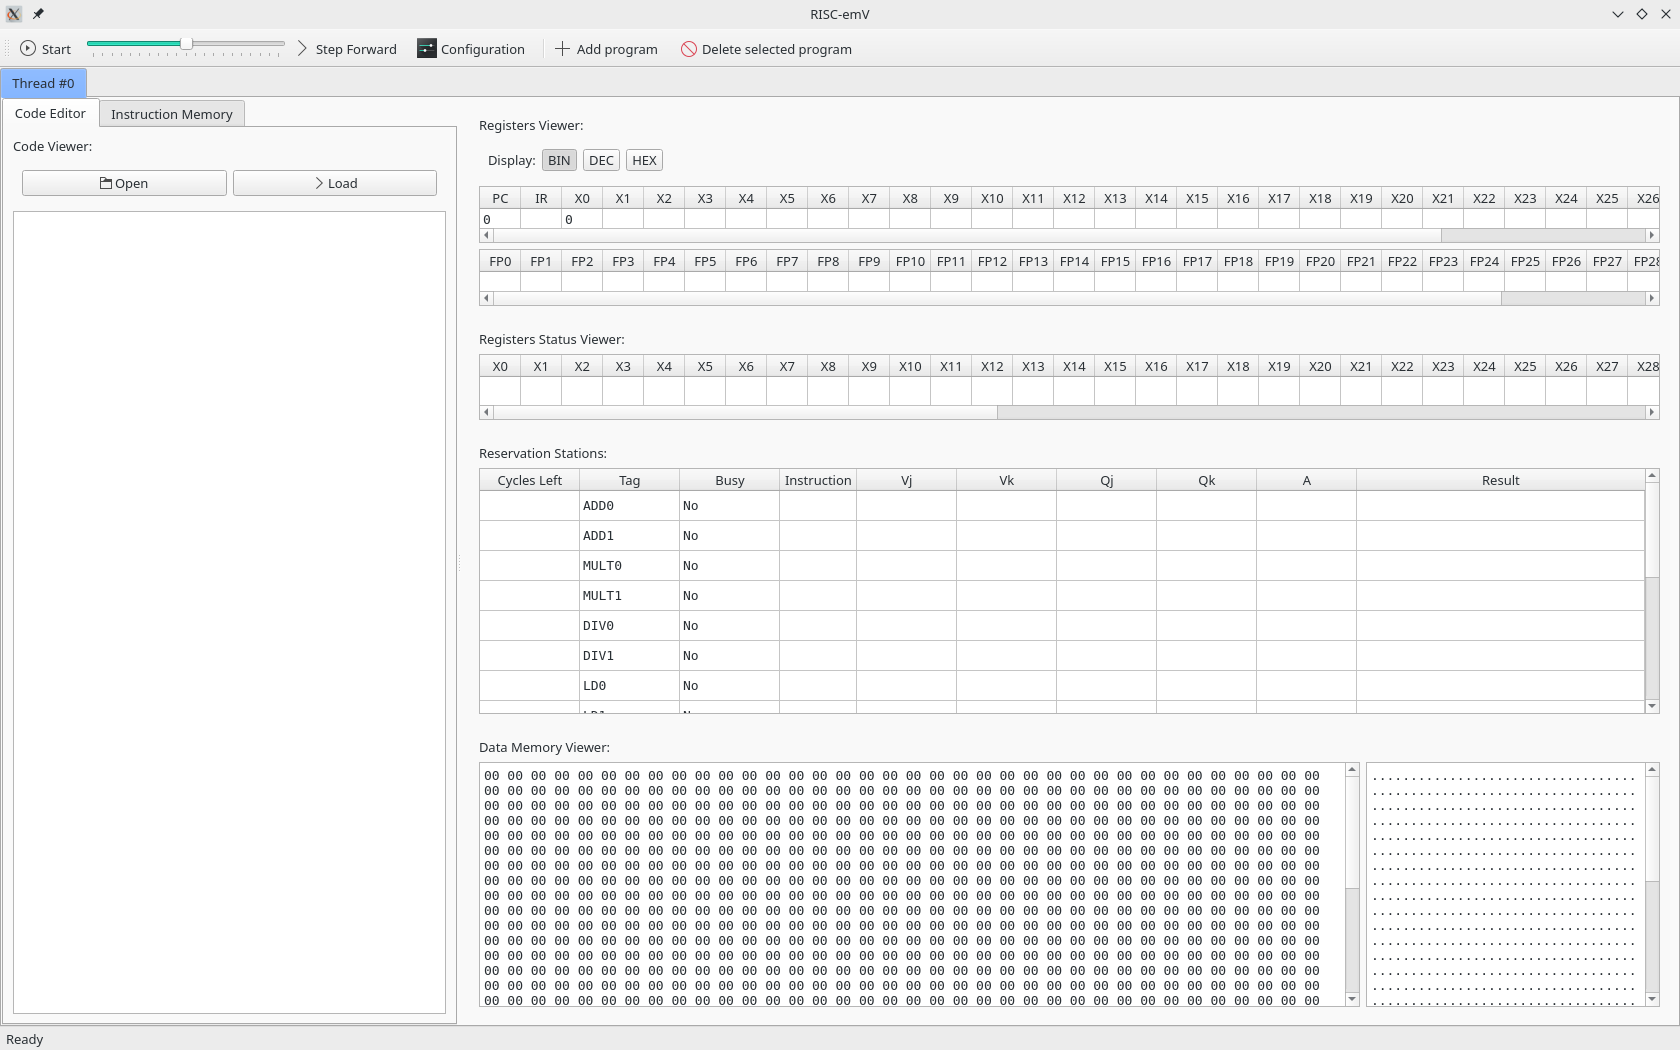
\includegraphics[width=\textwidth]{image_1.png}
\end{figure}

From top to bottom, the home screen contains a toolbar with the main emulator controls, a tab-bar to navigate and interact with the different threads (only one is loaded in the above screenshot), and an interface to the active thread’s components. A per-component description follows below:

\begin{itemize}
    \item \textbf{Toolbar}:
    \begin{itemize}
        \item \textbf{Start Emulator}: run the emulator executing one instruction after the other automatically
        \item \textbf{Step Delay}: delay to interleave between one instruction and the other
        \item \textbf{Step Forward}: perform one step and halt
        \item \textbf{Configuration}: open a configuration window to tune many parameters, such as number of functional units or per-instruction computation time in cycles. In the future it may hold more interesting possibilities such as the type of branch predictor to employ
        \item \textbf{Add thread}: create a new thread tab to load a program
        \item \textbf{Delete active thread}: delete the thread associated with the currently active thread tab
    \end{itemize}
    \item \textbf{Thread tab bar}: list of the currently active threads (with their associated colors for clarity). Clicking on one will update the frame below to match the thread’s execution environment
    \item \textbf{Emulator Components}:
    \begin{itemize}
        \item \textbf{Code text box}: read and edit the assembly code to be loaded and executed. The \textbf{open} button allows to import external \textbf{.s} and \textbf{.o} files, while the \textbf{load} button parses (or disassembles) the code and loads it into memory. This last step is necessary every time a new document is opened or a modification to the code is done, in order to update the process image in memory
        \item \textbf{Instruction Memory}: table of all loaded instructions with statistics on their timings when run (issue time, execution cycles, write-back time). In the future this section will allow the extraction of more detailed and informative reports about instruction frequency and functional units usage.
        \item \textbf{Registers}: interact with integer and floating point registers with the selected display format (binary, decimal, hexadecimal)
        \item \textbf{Registers Status}: inspect the status of registers, e.g. for which reservation station a register is waiting
        \item \textbf{Reservation Stations}: for each functional unit inspect its current instruction, data dependencies, and execution progress
        \item \textbf{Data Memory}: inspect the contents of the program’s memory, both in hexadecimal format and in ASCII characters
    \end{itemize}
\end{itemize}


\section{Source Code and Project Contents}
This project has been developed using \textbf{Python 3.x} and \textbf{PyQt5} for the GUI. The repository is structured in three main directories, containing the actual package (\hl{riscemv/}), a bunch of sample programs to play with (\hl{sample\_programs/}), and a collection of tests (\hl{tests/}) used during the development of the software to ensure the absence of regressions.\\

\noindent\hl{RISC-emV/}:
\begin{itemize}
    \item \hl{riscemv/}:
    \begin{itemize}
        \item Main implementation of the emulator architecture. \textbf{DataMemory.py}, \textbf{InstructionBuffer.py}, \textbf{RegisterFile.py}, \textbf{ReservationStations.py}, and \textbf{RegisterStatus.py} provide classes equivalent to their respective hardware elements, which are then collected and instantiated by the emulator object implemented in \textbf{Tomasulo.py}. Lastly, \textbf{Program.py} represents a process image, possibly generated by \textbf{ELF.py} if loaded from such format.
        \item \hl{gui/}:
        \begin{itemize}
            \item Files that generate the user interface. Many of these are the graphical counterparts of the previous mentioned classes, while \textbf{MainWindow.py} and \textbf{ConfWindow.py} serve as their respective windows launchers.
        \end{itemize}
        \item \hl{ISA/}:
        \begin{itemize}
            \item Implementation of the 7 types of RISC-V instructions (R, I, S, B, U, UJ, R4). Each of these types is available as a dedicated class, but all of them inherit common characteristics from a parent class contained in \textbf{Instruction.py}.
            \item \hl{Extensions/}:
            \begin{itemize}
                \item JSON files describing each ISA extension. Files in this folder are found and parsed automatically, and are composed of a list of instructions categorized by their type. Each instruction is represented as a JSON object containing its essential attributes, such as opcode, equivalent pseudocode, associated functional unit, etc.
            \end{itemize}
        \end{itemize}
    \end{itemize}
    \item \hl{sample\_programs/}:
    \begin{itemize}
        \item Ready to use assembly and object files, mainly carrying out very basic operations aimed at showcasing emulator’s functionalities without introducing real world programs’ structural complexities.
    \end{itemize}
    \item \hl{tests/}:
    \begin{itemize}
        \item Pytest-compatible tests, achieving (at the time of writing) 70\% code coverage. Continuous Integration was ensured thanks to TravisCI.
    \end{itemize}
\end{itemize}

\section{Challenges and Difficulties During Development}
A central challenge in projects with such a (somewhat) elevated number of classes and components is certainly proper synchronization and collaboration among teammates. Thanks to an appropriate use of version control systems and efficient communications, however, we managed to split work and responsibilities with great accuracy, so that every problem that arose was quickly traceable back to a source and an author that could efficiently take care of it.

Speaking of specific implementation challenges instead, support for ELF files proved to be quite a difficult feature to provide: although this format is very regular and easy to read thanks to the fixed-size tabular format, it has several fields with hard-to-comprehend meaning/purpose if one doesn’t have a thorough knowledge of the lifecycle of a source/program/process, as is our case.

Multithreading instead, we admit against our expectations, was only a matter of providing a means to instantiate a second emulator. This simplicity, as a matter of fact, was only allowed by the modularity we aimed to achieve from the beginning.

\section{Possible Future Advancements}
Thorough debugging might be considered our number one priority. This raises the need to extend current code testing to cover many more details, possibly including strict checks on data types, since in Python these are not enforced enough and often cause mismatches and unexpected type casts, leading for example to imprecise instruction outputs.

The strong modularity of this project also allows us to include in this list the development of further ISA extensions. For instance, RV32A to handle atomicity constraints to better handle multithreading, RV32C to support compressed instruction formats (RISC-V compilers currently default to this, unless otherwise requested), or more in general, implement 64 bit (or 128 bit, if confirmed in the near future) instruction parsing, which already meets partial support in the \textbf{ELF.py} class.

ELF file parsing could also see some improvements, such as proper parsing of linked programs, as currently it is only guaranteed to correctly parse relocatable programs.

Emulation of system calls and system libraries, in conclusion, would be another interesting feature, allowing for example a program to invoke I/O functions such as \textbf{printf} or \textbf{scanf} to interact with the user.


\end{document}
